\renewcommand{\this}{HMM_EM}

\chapter{Hidden Markov Models}

Talk about HMM use cases, sequential data, text processing, ... a bit outdated maybe.

\section{notation}
\begin{itemize}
\item $\mathcal{Z} = \{Z_1, ..., Z_T\}$: A random vector representing the categories, e.g. "verb".

\item $\mathcal{X} = \{X_1, ..., X_T\}$: A random vector representing the words, e.g. "work".

\item $\textbf{X}=\{x_1,...,x_T\}$: A \textbf{non-random} vector of \textbf{observations}, e.g a full scentence, note that $\textbf{X} \in O^T$.
		
\item $\textbf{Z}=\{z_1,...,z_T\}$: A \textbf{non-random} vector of \textbf{categories}, e.g a full scentence, note that $\textbf{Z} \in Q^T$.
		
\item $Q=\{q_1,...,q_K\}$: The collection of values $Z_i$ can take. Define $|Q|=K$.
		
\item $O=\{o_1,...,o_L\}$: The collection of words $X_i$ can take i.e. the corpus. Define $|O|=L$.

\item $A_{i\rightarrow j} = P(Z_t = q_j| Z_{t-1}=q_i)$: transition probability of going from category $i$ to category $j$. e.g. "Verb" $\to$ "Noun". Independent of $t$ since it's a markov chain.
		
\item $B_{i\rightarrow j} = P(X_t = o_j|Z_t = q_i)$: emission probability of emitting word $o_j$ if you're in category $i$. e.g. "Verb" $\to$ "work". Independent of $t$ since it's a markov chain.
		
\item $\theta$: collection of parameters $\theta = \{A_{ij,B_{ij}}, \pi\} \forall i,j$ here $\pi$ is the distribution of $Z_1$. i.e. Which "Adverb" is more likely as the category for the first word than "Verb".

\end{itemize}

Any hidden markov model can be represented as follows:
\begin{figure}[h!]
	\centering
	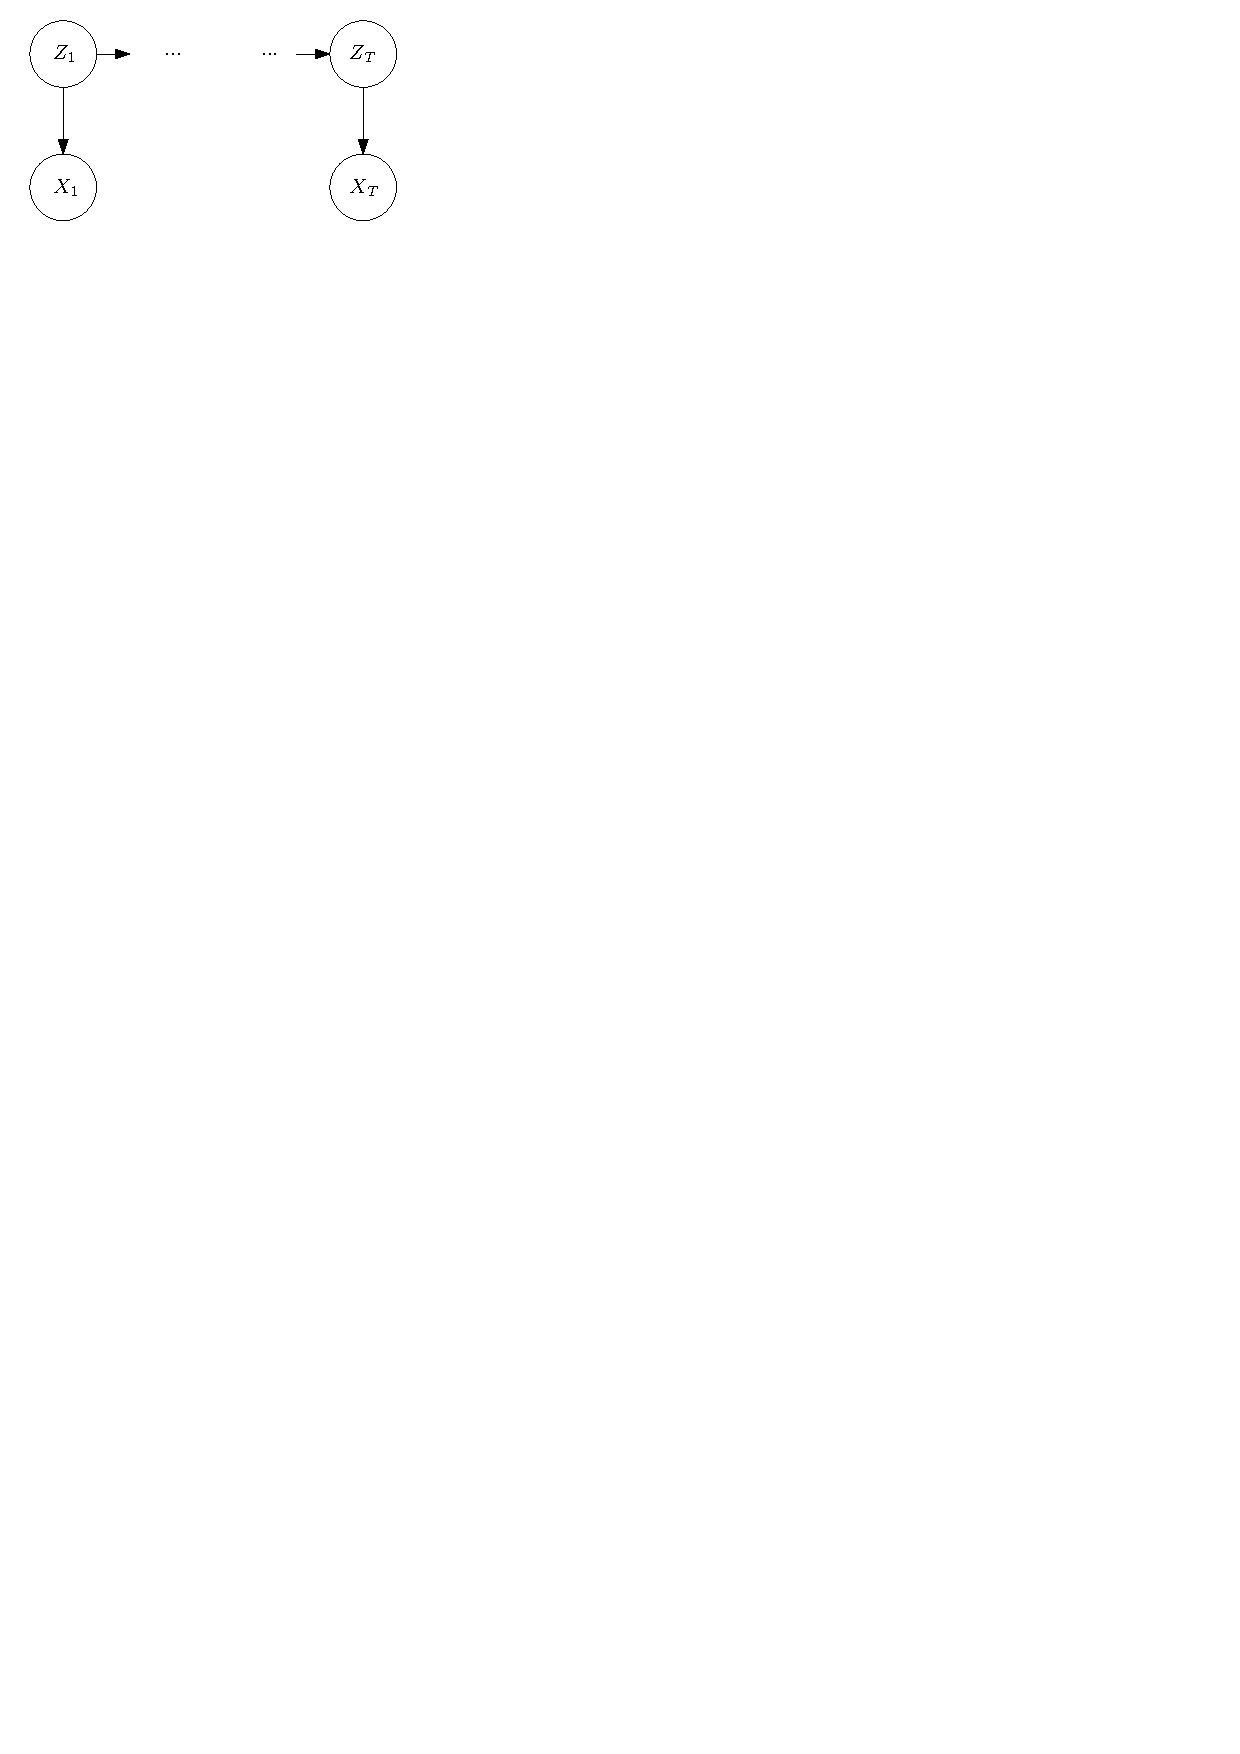
\includegraphics{\figDir/HMM.pdf}
\end{figure}
\section{Maximum likelihood for HMM}
\subsection{General principle of maximum likelihood}
	
Given data $\mathcal{X}$ that you assume comes from a probabilistic model $D \sim P(X|\theta)$. Maximum likelihood is a general principle in which you try to find parameters $\theta$ such that the data is "most likely" to occur. This means we find:

\begin{equation}
	\hat{\theta} = \underset{\theta}{\text{arg max }} P(D|\theta)
\end{equation}

However it is ofter easier to optimize the the $\log(.)$ of the likelihood function. Since $\log(.)$ is monotonically increasing minimizing this is by defninition identical, although often easier computationally.
\begin{equation}
	\hat{\theta} = \underset{\theta}{\text{arg max }} P(D|\theta) = \underset{\theta}{\text{arg max }} \log(P(D|\theta))
\end{equation}
	
I will denote the log liklihood as $L(D|\theta)$.\\\\

\textbf{Example:} Intuitively if we flip a coin 100 times and find 20 heads(=0) and 80(=1) tails. The parameter of this Bernouilli variable will more likely be higher than $p=0.5$.
	
\subsection{MLE for HMM}
\subsubsection{Likelihood of HMM}
Likelihood of a Hidden Markov Model is found by "pluggin in" bayesian network:
\begin{equation}
	\begin{split}
	P(\mathcal{Z},\mathcal{X}|\theta) &= \prod_{t=0}^{T-1}\underbrace{P(Z_{t+1}|Z_t)}_{transition}\underbrace{P(X_{t+1}|Z_{t+1})}_{emission}
	\end{split}
\end{equation}

Where $P(Z_1|Z_0) = P(Z_1)$, is the prior of the bayes net.
For hidden markov models we have addictional constraints on the parameters namely:
\begin{equation}
	\begin{split}
	\sum_{j=1}^{K}p(Z_{t+1} = q_j|Z_t = q_i)=\sum_{j=1}^{K} A_{i\rightarrow j} &= 1 \indent \forall i\\
	\sum_{j=1}^{L}p(X_{t} = o_j|Z_t = q_i)=\sum_{j=1}^{L} B_{i\rightarrow j} &= 1 \indent \forall i
	\end{split}
\end{equation}
	
Meaning that for every category in our set $Q$ the total probability of going to any state is 1 and the total probability of seeing any word should be 1.
	
\subsubsection{Small comment}
For HMM we can try to apply the maximum likelihood estimate. Since the likelihood for a HMM is given in terms of the observations $\textbf{X}=\{x_1,...,x_T\}$ and the known categories $\textbf{Z}=\{z_1,...,z_T\}$, in order to perform maximum likelihood we need both of these. This would for example mean that someone would categorise every word in a book before estimating the parameters, which some might consider impossible. However for now we assume this is no problem and continue.
	
\subsubsection{Actual calculation}
Almost all ML methods we will be maximizing the log-likelihood instead, note that in the following we no longer assume no data but instead assume observations $\textbf{X}$ and categories for these $\textbf{Z}$:
\begin{equation}
	\begin{split}
	\hat{\theta} = &\underset{A,B,\pi}{\text{arg max }}\log(\prod_{t=0}^{T-1}P(Z_{t+1} = z_{t+1}|Z_t=z_t)P(X_{t+1}=x_{t+1}|Z_{t+1}=z_{t+1}))\\
	&= \underset{A,B,\pi}{\text{arg max }} \sum_{t=0}^{T-1} log(P(Z_{t+1} = z_{t+1}|Z_t=z_t)) + \sum_{t=0}^{T-1} \log(P(X_{t+1}=x_{t+1}|Z_{t+1}=z_{t+1}))\\
	&=\underset{A,B,\pi}{\text{arg max }} \sum_{t=0}^{T-1} log(A_{t\rightarrow t+1}) + \sum_{t=0}^{T-1} \log(B_{t\rightarrow t})\\
	\end{split}		
\end{equation}
	
Note the notation it quite confusing at this point, however $A_{t\rightarrow t+1}$ is the probability of going from \textbf{observed} category at step $t$ in the chain to what we \textbf{observed} in step $t+1$. Same goes for $B_{t\rightarrow t}$.\\\\
So what's next? We know the parameters are optimal if the gradient w.r.t. the parameters is 0, i.e. $\nabla L(\textbf{X},\textbf{Z}|\theta) = 0$. However if we do this we overlooked a key component which are the extra constraints we placed on the parameters. A quick look at whet we maximize shows us that setting all parameters to $\infty$ is optimal, however clearly doesn't result in a proper transition or emission distribution. To include the constraints we use lagrange multipliers\footnote{Look at wikipedia for a quick guide, a really usefull trick to know in any field that uses any form of optimization: \url{https:// en.wikipedia.org/wiki/Lagrange_multiplier}}:
\begin{equation}
	\mathcal{L}(\theta, \lambda, \alpha) = \sum_{t=0}^{T-1} log(A_{t\rightarrow t+1}) + \sum_{t=0}^{T-1} \log(B_{t\rightarrow t})\\
	+\sum_{i}^{K}\lambda_i(1-\sum_{j}^{K}A_{i\rightarrow j}) +\sum_{i}^{K}\alpha_i(1-\sum_{j}^{L}B_{i \rightarrow j})
\end{equation}
The above function is called the lagrangian. Now all we have to do is optimize this. Since the general lagrange theory says that for optimal solution $\hat{\theta}$ of the constrained problem, there exists $\hat{\lambda}$ and $\hat{\alpha}$ such that $(\hat{\theta},\hat{\lambda}, \hat{\alpha})$ is a stationary point of $\mathcal{L}(\theta, \lambda, \alpha)$. In short, we can maximize $\mathcal{L}(\theta, \lambda, \alpha)$ and find $\lambda$ and $\alpha$ instead of doing constrained optimization. First we find the the optimal transtion parameters, the emission parameters are identical by symmetry of the lagrangian.
\begin{equation}
		\begin{split}		
		\frac{\partial}{\partial A_{f\rightarrow s}}\mathcal{L}(\theta, \lambda, \alpha) =& \frac{\partial}{\partial A_{f\rightarrow s}}\left(\sum_{t=0}^{T-1} log(A_{t\rightarrow t+1})\right) + \sum_{t=0}^{T-1}0 + \frac{\partial}{\partial A_{f\rightarrow s}}\left( \sum_{i}^{K}\lambda_i(1-\sum_{j}^{K}A_{i\rightarrow j})\right)+\sum_{i=0}^{K}0\\
		=&  \left(\sum_{t=0}^{T-1} \frac{\mathbbm{1}[x = A_{f\rightarrow s}](A_{t\rightarrow t+1})}{A_{f\rightarrow s}}\right) - \lambda_{f}
		\end{split}
\end{equation}

To derive the lagrangian we see that the components which do not contain $A_{f\rightarrow s}$ derive to $0$. In the first sum only the observations of $A_{f\rightarrow s}$, i.e. when we observe going from category $f$ to $s$., will derive to $\frac{\partial}{\partial A_{fs}} \log A_{f\rightarrow s} = \frac{1}{A_{f\rightarrow s}}$. Hence the indicator function $\mathbbm{1}[x = A_{f\rightarrow s}](A_{t\rightarrow t+1})$, it is $0$ when the input $A_{t\rightarrow t+1}$ is not $A_{f\rightarrow s}$. Now setting the derivative to zero to find optimality:

\begin{equation}
	\begin{split}
	\left(\sum_{t=0}^{T-1} \frac{\mathbbm{1}[x = A_{f\rightarrow s}](A_{t\rightarrow t+1})}{A_{f\rightarrow s}}\right) - \lambda_{f} &= 0\\
	\frac{count(f\rightarrow s)}{A_{f\rightarrow s}} &= \lambda_f\\
	A_{f\rightarrow s} &= \frac{count({f\rightarrow s})}{\lambda_{f}}
	\end{split}
\end{equation}
	
However now we need to find what $\lambda_f$ is. We do this by enforcing the transition constraint, that is from any category $f$ we must go to any other state $s$. In formula we want $\sum_{j=1}^{K} A_{i\rightarrow j} = 1 \indent \forall i$:
\begin{equation}
	\begin{split}
	\sum_{j=1}^{K} A_{i\rightarrow j} &= 1\\
	\sum_{j=1}^{K} \frac{count({f\rightarrow j})}{\lambda_{f}} &= 1\\
	\sum_{j=1}^{K} count({f\rightarrow j}) &= \lambda_f
	\end{split}
\end{equation}
	
We find $\lambda_f$ to be the total amount of time a transition starting in $f$ is observed. We find the estimate of $A_{fs}$ simply as the fraction:

\begin{equation}
	\hat{A}_{f\rightarrow s} = \frac{count({f\rightarrow s})}{\sum_{j=1}^{K} count({f\rightarrow j})}
\end{equation}
	
The fraction of times you observe a transition from $f$ to $s$ compared to the total amount of times a transition from $f$ to any state is observed.
\\\\
Note by looking at the lagrangian we find symmetry and the maximum likelihood estimate of $B_{fo}$ can be derived in exactly the same way as the maximum likelihood for $A_{fs}$, resulting in:

\begin{equation}
	\hat{B}_{fo} = \frac{count({f\rightarrow o})}{\sum_{o=1}^{L}count({f\rightarrow o})}
\end{equation}

Again the notation doesn't work out very nice, however it explains the situation. Again the maximum likelihood estimate for observing word $o$ given category $f$ is the fraction of times we observe $o$ in category $f$ compared to the amount of times we observe category $f$. Note a special case is $A_{0j}$ which is then simply the fraction of times we observe category $j$ compared to the rest of the categories.

\section{EM for HMM}
Expectation maximization is a general and widely used algorithm in machine learning to deal with either missing data or unobserved/latent variables to maximize the parameters of a model. It does this by estimating the likelihood iteratively and adapting the parameters.

\subsection{EM in \textbf{general}}
This part is based on the wikipedia article on EM\footnote{\url{https://en.wikipedia.org/wiki/Expectation_maximization_algorithm}}. Note that I use the same notation of the wikipedia article, $\textbf{Z}$ does not denote categories in a HMM nor does $\textbf{X}$ represent observations. In fact in the following we don't even assume that our model is a HMM.
Say we have a statistical model that generates $\textbf{X}$ observed data and $\textbf{Z}$ unobserved data. This model is parameterized by \textbf{$\theta$}, then the likelihood of this observed/unobserved data is defined as:
\begin{equation}
\begin{split}
L(\theta;\textbf{X}) &= \sum_{z} L(\theta;\textbf{X},z)\\
&= \int_{Z}L(\theta;\textbf{X},z)dz
\end{split}
\end{equation}
We could try to maximize this quantity over $\theta$, and this would work perfectly fine. However, this often proves intractable since we have to sum/integrate over $Z$.\\

Since this is intractable, in practice the EM algorithm is used instead. The EM algorithm consists of the following 2 steps:
\begin{equation}
Q(\theta|\theta^{(t)}) = \mathbb{E}_{\textbf{Z}|\textbf{X}, \theta^{(t)}}[\log L(\theta;\textbf{X},\textbf{Z})]
\end{equation}
Which is the expectation over $\textbf{Z}$ given observed data $\textbf{X}$ and previous $\theta^{(t)}$ of the log-likelihood of observed and unobserved data. This is called the \textbf{Expectation} step.
\begin{equation}
\theta^{(t+1)} = \underset{\theta}{\text{arg max }} Q(\theta|\theta^{(t)}) 
\end{equation}
The update for $\theta^{(t)}$ is the maximization of $Q$. This is called the \textbf{Maximization} step.
\pagebreak
\subsection{EM for HMM}
We can apply EM for HMM, in previous section I tried to emphasise the fact that $\textbf{Z}$ just denoted variables we don't know or are latent and not specifically the categories of a HMM. However in the case of HMM $\mathcal{Z}$ actually are the latent variables. Aswell as $\mathcal{X}$ being the observed variables.
\subsubsection{Expectation in HMM}
Plugging in the definition using the log liklihood of HMM and the definition of expectation for discrete variables we find:
\begin{equation}
\begin{split}
\mathbb{E}_{\textbf{Z}|\textbf{X}, \theta^{(t)}}[\log L(\theta;\textbf{X},\textbf{Z})] &= \sum_{\textbf{Z}}p(\textbf{Z}|\textbf{X},\theta^{(t)})\left(\sum_{t=0}^{T-1} log(A_{t,t+1}) + \sum_{t=0}^{T-1} \log(B_{tt}) \right)\\
=& \sum_{\textbf{Z}}p(\mathbf{Z}|\mathbf{X},\theta^{}(t))log(A_{0,1}) + ... + \sum_{\textbf{Z}}p(\mathbf{Z}|\mathbf{X},\theta^{}(t))log(A_{T-1,T}) \\&+ \sum_{\textbf{Z}}p(\mathbf{Z}|\mathbf{X},\theta^{}(t))log(B_{11})\\
\end{split}
\end{equation}
Note thet we are summing over $\textbf{Z}$, this is the vector of categories in each timestep. More formally we can actually write:
\begin{equation}
\sum_{\textbf{Z}} = \sum_{z_1}\sum_{z_2}...\sum_{z_T}
\end{equation}
In order to make life easier we look at what happens to a single term of the form $log(A_{t,t+1})$ by taking the sum inside, more concretely what I mean is the following:
\begin{equation}
\begin{split}
\sum_{z_1}\sum_{z_2}...\sum_{z_T}p(z_1,...,z_T|\mathbf{X},\theta^{(t)})log(A_{i,i+1})
\end{split}
\end{equation}
\end{document} 
